\documentclass[12pt,letterpaper]{book}
\usepackage[a4paper,width=15cm,top=2.5cm,bottom=2.5cm,bindingoffset=6mm]{geometry}
\usepackage{footnote}
\usepackage{amsbsy}
\usepackage{amsmath}
\usepackage{physics}
\usepackage{graphicx}
\usepackage{fancyhdr}
\usepackage[T1]{fontenc} % important for having seachable underscores
\usepackage{bm}
\usepackage[sort&compress,numbers]{natbib}
\setlength{\parskip}{2.54mm}


\usepackage{color}
\def\red{\textcolor{red}}
\def\old#1{\textcolor{red}{#1}}
\def\new#1{\textcolor{blue}{#1}}

% Print only chapters in the Table Of Contents
\setcounter{secnumdepth}{2}
\setcounter{tocdepth}{2} 

% Ensure that blank pages don't have numbers or heading on them 
\makeatletter
\def\cleardoublepage{\clearpage\if@twoside \ifodd\c@page\else
 \hbox{}
 \vspace*{\fill}
 \thispagestyle{empty}
 \newpage\fi\fi}
\makeatother

% set fancy headings
\pagestyle{fancy}
\lhead[{\it \thepage}]{{\bf\it Research Notes}}
\chead{}
\rhead[{\bf\it Research Notes}]{{\it \thepage}}
\renewcommand{\headrulewidth}{0.2pt}
\lfoot{}
\cfoot{}
\rfoot{}
\renewcommand{\footrulewidth}{0pt}
\setlength{\footskip}{0.25in}
\setlength{\parindent}{0in}

%% This part slightly modifies the default definition of \chapter
%% (found in book.cls) to add a \hspace{2em} before numbered chapters.
\makeatletter
\def\@chapter[#1]#2{\ifnum \c@secnumdepth >\m@ne
                       \if@mainmatter
                         \refstepcounter{chapter}%
                         \typeout{\@chapapp\space\thechapter.}%
                         \addcontentsline{toc}{chapter}%
                                   {\hspace{2em}\protect\numberline{\thechapter}#1}%
                       \else
                         \addcontentsline{toc}{chapter}{#1}%
                       \fi
                    \else
                      \addcontentsline{toc}{chapter}{#1}%
                    \fi
                    \chaptermark{#1}%
                    \addtocontents{lof}{\protect\addvspace{10\p@}}%
                    \addtocontents{lot}{\protect\addvspace{10\p@}}%
                    \if@twocolumn
                      \@topnewpage[\@makechapterhead{#2}]%
                    \else
                      \@makechapterhead{#2}%
                      \@afterheading
                    \fi}
\makeatother


% reset vec and hat style to a bold type
\let\oldhat\hat
\renewcommand{\hat}[1]{\oldhat{\mathbf{#1}}}
\renewcommand{\vec}[1]{\mathbf{#1}}
% stretches the vertical spacing of arrays/matrices
\renewcommand{\arraystretch}{2}
\setlength{\jot}{10pt}

\graphicspath{ {./images/} }
\title{Research Notes}
\author{Aidan Winblad}
\date{\today}
%%% THIS SHOULD BE THE LAST PACKAGE TO BE LOADED!
%hidelinks to remove colored borders from links
%plainpages=false needed for the unnumbered pages
%breaklinks=true to allow to break long links (e.g. long titles) on
%more than one line
%bookmarksopen open the bookmarks in the adobe reader plugin
%bookmarksopenlevel decide the max level at which the bookmarks should
%be open
% pdfdisplaydoctitle=true to show the document title instead of the
% filename in the titlebar of adobereader
\usepackage[plainpages=false,breaklinks=true,pdfborder=0 0 0,pdfdisplaydoctitle=true,bookmarksopen=true,bookmarksopenlevel=0,pdftex,%
%Comment next line if it makes problems
%(it requires a recent LaTeX distribution)
            hidelinks,
            pdftitle={MSE502B},
            pdfkeywords={lecture notes}]{hyperref}


\begin{document}

\maketitle
\tableofcontents

%\chapter{Solving the Bogoliubov-de Gennes Hamiltonian for a triangular lattice}
\section{Finite lattice real space}
The Bogoliubov-de Gennes (BdG) Hamiltonian is commonly used for describing quasiparticle excitations in superconductors. In this work we will solve the BdG equation for a topological  superconductor on an equilateral triangle of finite lattice sites. An equilateral triangle is chosen because it is topologically equivalent to a T-junction which is commonly used for illustrating braiding operations of Majorana fermions in 1D topological superconductors. 

We solve the system numerically for finite lattice sites. Begin by starting with the tight-binding Hamiltonian for a $\vec{p}$-wave superconductor on a triangular lattice
\begin{equation}
\mathcal{H} = \sum\limits_{i} (6t-\mu)c^{\dagger}_{i}c_{i} + \sum\limits_{<i,j>} \left(-tc^{\dagger}_{i}c_{j} + \Delta e^{i\phi_{ij}}c^{\dagger}_{i}c^{\dagger}_{j} + h.c.\right).
\end{equation}

To get to the BdG Hamiltonian we need to use the anticommutation relation for fermions
\begin{align}
\{c_i,c_j\} &= \{c_i^\dagger,c_j^\dagger\} = 0 \\
\{c_i^\dagger,c_j\} &= c_i^\dagger c_j + c_j c_i^\dagger = \delta_{ij},
\end{align}

Which allows us to write the operators as
\begin{align}
c_i^\dagger c_j &= \frac{1}{2}(c_i^\dagger c_j - c_j c_i^\dagger + \delta_{ij}) \\
c_i c_j &= \frac{1}{2}(c_i c_j - c_j c_i ).
\end{align}

Using the Nambu spinor in lattice space and momentum space
\begin{align}
  \Psi &\equiv (c_1,\cdots,c_N,c_1^\dagger,\cdots,c_N^\dagger)^T \\
  \Psi &\equiv (c_k, c_{-k}^\dagger)^T
\end{align}

We can rewrite the tight-binding Hamiltonian as
\begin{equation}
\mathcal{H} = \frac{1}{2}\Psi^{\dagger}H_{BdG}\Psi.
\label{eqn=CompactHamiltonian}
\end{equation}

The HdG Hamiltonian is then solved numerically using a python script (REFERENCE SRC HERE). 
\section{Infinite lattice momentum space}
We then solve our problem in momentum space for an infinite triangular lattice. Starting back at the tight-binding Hamiltonian we take the fourier transform of the creation and annihilation operators where
\begin{equation}
  c_i = \frac{1}{\sqrt{N}} \sum\limits_{\vec{k}} c_k e^{-i\vec{k}\cdot\vec{r_i}}.
\end{equation}

Following the sames steps as mentioned before we arrive at the same compact form as Eqn. \ref{eqn=CompactHamiltonian} where the BdG Hamiltonian is simply a $2\times2$ matrix 

\[
H_{BdG}=
  \begin{bmatrix}
   t(\vec{k}) & \Delta(\vec{k})\\
   \Delta^{\star}(\vec{k}) & -t(\vec{k})
  \end{bmatrix}.
\]

The functions of the BdG matrix are 
\begin{align}
t(\vec{k}) &= -2t\left[\cos(ak_x) + \cos\left(\frac{ak_x}{2}+\frac{\sqrt{3}ak_y}{2}\right) + \cos\left(\frac{ak_x}{2}-\frac{\sqrt{3}ak_y}{2}\right)\right] - (\mu - 6t) \\
\Delta(\vec{k}) &= 2\Delta i \left[\sin(ak_x)-e^{\frac{4\pi i}{3}}\sin\left(\frac{ak_x}{2}+\frac{\sqrt{3}ak_y}{2}\right) + e^{\frac{5\pi i}{3}}\sin\left(\frac{ak_x}{2}-\frac{\sqrt{3}ak_y}{2}\right)  \right]
\end{align}

The determinant of this matrix is easily solved to give the energy eigenvalues as $E = \pm\sqrt{t(\vec{k})^2 + \|\Delta(\vec{k})\|^2 }$.

\section{Results}
NEED TO FINISH THIS SECTION (FIXED THE FIGURE LABELS OF THE FIGURES AND REFERENCES)
The numerical approach to solving the finite triangle has some hangups. The BdG Hamiltonian is of the size $ 2N \times 2N $ and eigenvalue solvers run on the order of $\mathcal{O}(n^3)$. This severly dampens the ability to simulate a physically realizable triangular lattice. Aside from that we can still get meaningful physical phenomena from using a small triangular lattice. Let us first look at the energy spectra of both the finite lattice in real space and infinite lattice in momentum space. The momentum energy spectra seen in Fig. \ref{fig-momspectra} shows an apparent energy band gap of $\Delta\epsilon = \pm2(t)$ while the real space energy spectra in Fig \ref{fig-enespectra} shows energy values lying within the energy band gap.

\begin{figure}
%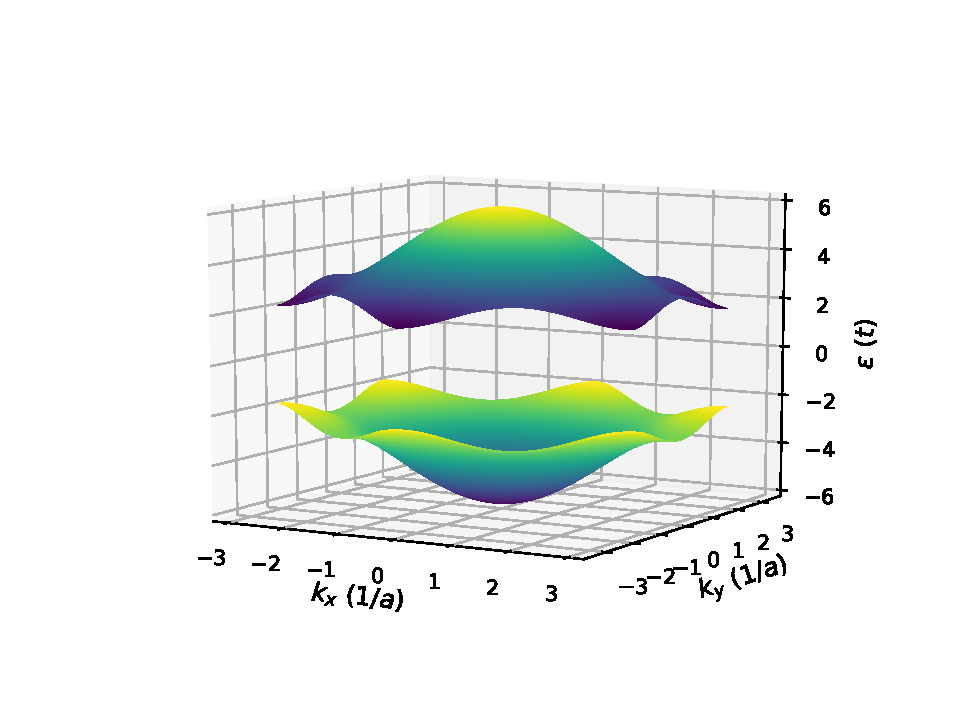
\includegraphics[scale=.5]{fig-energy-band-gap-momentum-space.pdf}
\caption{}
\label{fig-momspectra}
\end{figure}

\begin{figure}
%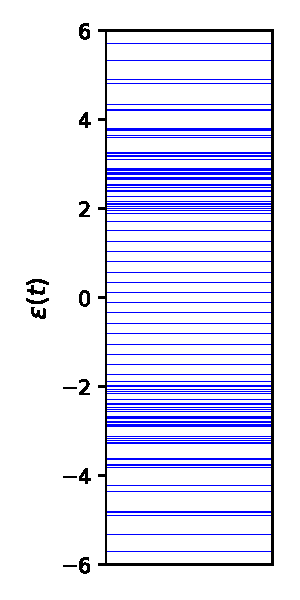
\includegraphics[scale=.5]{fig-energy-spectra.pdf}
\caption{}
\label{fig-enespectra}
\end{figure}

\begin{figure}
%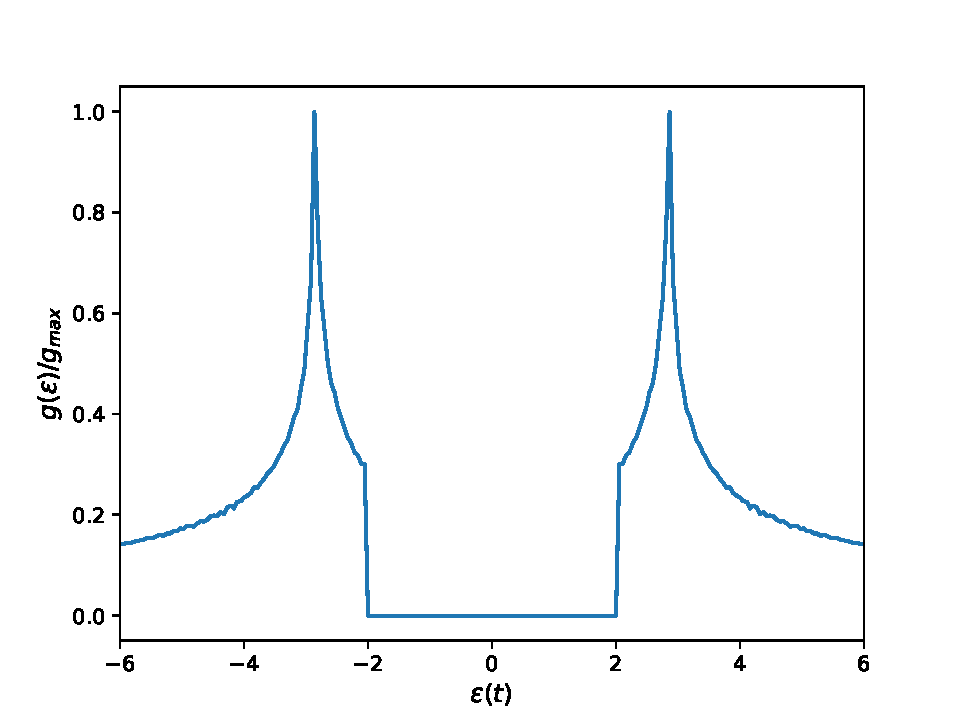
\includegraphics[scale=.5]{fig-dos-momentum.pdf}
\caption{}
\label{fig-dosmom}
\end{figure}

\begin{figure}
%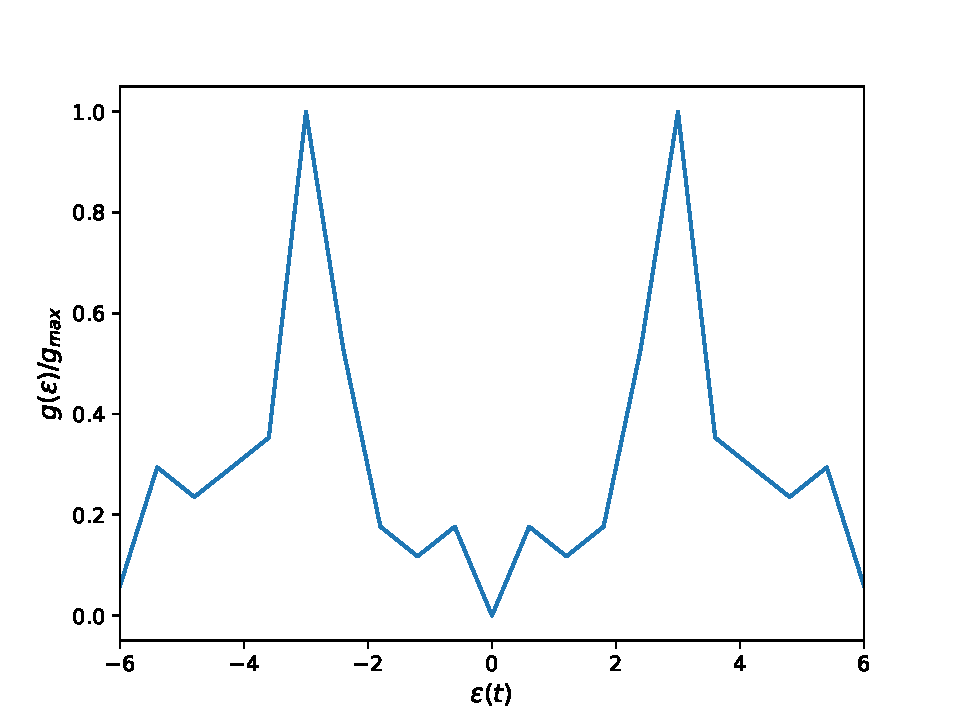
\includegraphics[scale=.5]{fig-dos-real-space.pdf}
\caption{}
\label{fig-dosspace}
\end{figure}




%\chapter{Majorana fermions in a tunable semiconductor device}
\section{Applying an on axis Magnetic Field}

A method for making a Majorana fermion tunable device has been shown in two forms, one by D. Sau (REFERENCE) and J. Alicea (REFERENCE). A zinc-blende semiconductor quantum well grown along the (100) direction is considered. We start with the relevant noninteracting Hamiltonian

\begin{equation}
  \mathcal{H}_0 = \sum\limits_{\vec{k}} c_{\vec{k}}^\dagger \left[\frac{k^2}{2m} - \mu + \alpha ( \sigma^x k_y - \sigma^y k_x) \right] c_{\vec{k}}
\end{equation}
where $m$ is the effective mass, $\mu$ is the chemical potential, $\alpha$ is the Rashba spin-orbit(REFERENCED in Alicea's paper as ref 23) coupling strength, and $\sigma^i$ are the Pauli matrices that act on the spin degrees of freedom in $c_{\vec{k}}$. We have set $\hbar=1$ throughout.

We next introduce a ferromagnetic insulator and a magnetic field. The ferromagnetic insulator has magnetization pointing perpendicular to the 2D semiconductor. While the magnetic field will point parallel to the 2D  semiconductor. We assume this will induce a Zeeman interaction

\begin{equation}
  \mathcal{H}_Z = \sum\limits_{\vec{k}} c_{\vec{k}}^\dagger \left[V_x \sigma^x + V_y \sigma^y + V_z \sigma^z \right] c_{\vec{k}}
\end{equation}
but neglible orbital coupling. If we look at the combined Hamiltonian it becomes obvious there is a constant energy plus the energy eigenvalues of the Pauli matrices terms. We can easily solve the eigenvalue problem of

\begin{equation}
  \begin{bmatrix}
    V_z & V_x + \alpha k_y - i(V_y - \alpha k_x) \\
    V_x + \alpha k_y + i(V_y -\alpha k_x) & -V_z
  \end{bmatrix}
\end{equation}

or in a more compact form using $\beta(\vec{k}) = k_y + V_x/\alpha$ and $\gamma(\vec{k}) = k_x - V_y/\alpha$ and $\eta^2(\vec{k})=\beta^2(\vec{k})+\gamma^2(\vec{k})$ and we produce

\begin{equation}
  \begin{bmatrix}
    V_z    &    \alpha(\beta(\vec{k}) + i\gamma(\vec{k})) \\
    \alpha(\beta(\vec{k}) - i\gamma(\vec{k})) &    -V_z
  \end{bmatrix}
\end{equation}

giving $\epsilon_{\pm}' = \pm \sqrt{V_z^2+\alpha^2\eta^2(\vec{k})}$ with eigenvectors

\begin{align}
  u_+(\vec{k})  =  
  \left( \begin{array}{l}
      A_\uparrow(\vec{k}) \\ 
      -A_\downarrow(\vec{k}) \dfrac{\beta(\vec{k}) - i \gamma(\vec{k})}{\eta(\vec{k})}
  \end{array} \right)
  \\ \\
  u_-(\vec{k})  =  
  \left( \begin{array}{l}
      B_\uparrow(\vec{k}) \dfrac{\beta(\vec{k}) + i \gamma(\vec{k})}{\eta(\vec{k})}  \\ 
      B_\downarrow(\vec{k})
  \end{array} \right)
\end{align}

One can find $A_{\sigma}=A_{\sigma}^*$ and $B_{\sigma}=B_{\sigma}^*$ and the coefficients are

\begin{align}
  A_{\uparrow}(\vec{k}) &= \dfrac{-\alpha\eta(\vec{k})}{\sqrt{2\epsilon_+'(\vec{k})}} \sqrt{\dfrac{1}{\epsilon_+'(\vec{k})-V_z}} \\
A_{\downarrow}(\vec{k}) &= \sqrt{\dfrac{\epsilon_+'(\vec{k})-V_z}{2\epsilon_+'(\vec{k})}} \\
B_{\uparrow}(\vec{k}) &= \sqrt{\dfrac{\epsilon_-'(\vec{k})+V_z}{2\epsilon_-'(\vec{k})}} \\ 
B_{\downarrow}(\vec{k}) &= \dfrac{\alpha\eta(\vec{k})}{\sqrt{2\epsilon_-'(\vec{k})}} \sqrt{\dfrac{1}{\epsilon_-'(\vec{k})+V_z}}
\end{align}

If in the case of $V_x=V_y=0$ we arrive back at solution Sau $\mathit{et\ al.}$ calculate for eigenvalues, vectors, and coefficients. The expressions for $A_{\uparrow,\downarrow}$ and $B_{\uparrow,\downarrow}$ can be written in convenient terms as

\begin{align}
  f_p(\vec{k}) &= A_{\uparrow}(\vec{k})A_{\downarrow}(-\vec{k}) = B_{\uparrow}(-\vec{k})B_{\downarrow}(\vec{k}) \\
  &= \dfrac{-\alpha \eta(\vec{k})}{2\sqrt{\epsilon_+'(\vec{k})\epsilon_+'(-\vec{k})}} \sqrt{\dfrac{\epsilon_+'(-\vec{k})-V_z}{\epsilon_+'(\vec{k})-V_z}}
\end{align}

When putting the semiconductor in contact with an $s$-wave superconductor a pairing term is generated by the proximity effect. The full Hamiltonian becomes $\mathcal{H} = \mathcal{H}_0 + \mathcal{H}_Z + \mathcal{H}_{SC}$ with

\begin{align}
  \mathcal{H}_{SC} = \sum\limits_{\vec{k}} \Delta c_{\uparrow,\vec{k}}^\dagger c_{\downarrow,-\vec{k}}^\dagger + H.c.
\end{align}

We now want to write the pairing potential in terms of $c_{\pm}$ using a basis transformation.

\begin{align}
  c_{\uparrow,\vec{k}} &= \bra{\uparrow}\ket{u_+(\vec{k})} c_{\vec{k},+} + \bra{\uparrow}\ket{u_-(\vec{k})} c_{\vec{k},-} \\
  &= A_{\uparrow}(\vec{k}) c_{\vec{k},+} + B_{\uparrow}(\vec{k})\dfrac{\beta(\vec{k})+i\gamma(\vec{k})}{\eta(\vec{k})} c_{\vec{k},-} \\
  c_{\downarrow,-\vec{k}} &= \bra{\downarrow}\ket{u_+(-\vec{k})} c_{-\vec{k},+} + \bra{\downarrow}\ket{u_-(-\vec{k})} c_{-\vec{k},-} \\
  &= -A_{\downarrow}(-\vec{k})\dfrac{\beta(-\vec{k})-i\gamma(-\vec{k})}{\eta(-\vec{k})} c_{-\vec{k},+} + B_{\downarrow}(-\vec{k}) c_{-\vec{k},-}
\end{align}

with the adjoints being
\begin{align}
  c_{\uparrow,\vec{k}}^{\dagger} &= A_{\uparrow}(\vec{k}) c_{\vec{k},+}^{\dagger} + B_{\uparrow}(\vec{k})\dfrac{\beta(\vec{k})-i\gamma(\vec{k})}{\eta(\vec{k})} c_{\vec{k},-}^{\dagger} \\
  c_{\downarrow,-\vec{k}}^{\dagger} &= -A_{\downarrow}(-\vec{k})\dfrac{\beta(-\vec{k})+i\gamma(-\vec{k})}{\eta(-\vec{k})} c_{-\vec{k},+}^{\dagger} + B_{\downarrow}(-\vec{k}) c_{-\vec{k},-}^{\dagger}
\end{align}

Continue reducing the pairing potential which becomes

\begin{equation}
  \begin{split}
    \Delta c_{\uparrow,\vec{k}}^{\dagger}c_{\downarrow,-\vec{k}}^{\dagger}  = \Delta &[ -A_{\uparrow}(\vec{k})A_{\downarrow}(-\vec{k})\dfrac{\beta(-\vec{k})+i\gamma(-\vec{k})}{\eta(-\vec{k})}c_{\vec{k},+}^{\dagger}c_{-\vec{k},+}^{\dagger} \\
    + & B_{\uparrow}(\vec{k})B_{\downarrow}(-\vec{k})\dfrac{\beta(\vec{k})-i\gamma(\vec{k})}{\eta(\vec{k})}c_{\vec{k},-}^{\dagger}c_{-\vec{k},-}^{\dagger}  \\
  +&\left(A_{\uparrow}(\vec{k})B_{\downarrow}(-\vec{k})-B_{\uparrow}(\vec{k})A_{\downarrow}(-\vec{k})\dfrac{\beta(\vec{k})-i\gamma(\vec{k})}{\eta(\vec{k})}\dfrac{\beta(-\vec{k})+i\gamma(-\vec{k})}{\eta(-\vec{k})} \right) c_{\vec{k},+}^{\dagger}c_{-\vec{k},-}^{\dagger} ]
  \end{split}
\end{equation}

We will use a more convenient notation by making the following substitutions

\begin{align}
  \Delta_{++}(\vec{k}) &= -\Delta f_p(\vec{k}) \dfrac{\beta(-\vec{k}) +i\gamma(-\vec{k})}{\eta(-\vec{k})} \\
  \Delta_{--}(\vec{k}) &= \Delta f_p(-\vec{k}) \dfrac{\beta(\vec{k}) -i\gamma(\vec{k})}{\eta(\vec{k})} \\
  \Delta_{+-}(\vec{k}) &= \Delta f_s(\vec{k})
\end{align}

Where 

\begin{align}
  f_s(\vec{k}) = \left(A_{\uparrow}(\vec{k})B_{\downarrow}(-\vec{k})-B_{\uparrow}(\vec{k})A_{\downarrow}(-\vec{k})\dfrac{\beta(\vec{k})-i\gamma(\vec{k})}{\eta(\vec{k})}\dfrac{\beta(-\vec{k})+i\gamma(-\vec{k})}{\eta(-\vec{k})} \right)
\end{align}

The pairing potential Hamiltonian then becomes

\begin{align}
  \mathcal{H}_{SC} = \sum\limits_{\vec{k}} \Delta_{++}c_{\vec{k},+}^{\dagger}c_{-\vec{k},+}^{\dagger} + \Delta_{--}c_{\vec{k},-}^{\dagger}c_{-\vec{k},-}^{\dagger} +\Delta_{+-}c_{\vec{k},+}^{\dagger}c_{-\vec{k},-}^{\dagger} + H.c.
\end{align}

Writing the full Hamiltonian in compact form we will use the following Nambu spinor

\begin{align}
  \Psi = (c_{\vec{k},+},\ c_{\vec{k},-},\ c_{-\vec{k},+}^{\dagger},\ c_{-\vec{k},-}^{\dagger} )^T
\end{align}

Then we write the Hamiltonian as, where we have used the conventional BdG approach of applying the anticommutation relation and reindexing the momentum vetor of the second term to give

\begin{align}
  \mathcal{H} = \dfrac{1}{2}\sum\limits_{\vec{k}} \Psi^{\dagger}H_{BdG}\Psi
\end{align}

with 

\begin{equation}
  H_{BdG} = 
  \begin{bmatrix}
    \epsilon_+(\vec{k}) & 0 & 2\Delta_{++}(\vec{k}) & \Delta_{+-}(\vec{k}) \\
    0 & \epsilon_-(\vec{k}) & -\Delta_{+-}(-\vec{k}) & 2\Delta_{--}(\vec{k}) \\
    2\Delta_{++}^*(\vec{k}) & -\Delta_{+-}^*(-\vec{k}) & -\epsilon_+(-\vec{k}) & 0 \\
    \Delta_{+-}^*(\vec{k}) & 2\Delta_{--}^*(\vec{k}) & 0 & -\epsilon_-(-\vec{k}) \\
  \end{bmatrix}
\end{equation}

where 

\begin{equation}
  \epsilon_{\pm}(\vec{k}) = \dfrac{k^2}{2m} - \mu + \epsilon_{\pm}'(\vec{k})
\end{equation}

We can rearrange our matrix into a more block diagonal form with off terms to give

\begin{equation}
  H_{BdG} = 
  \begin{bmatrix}
    \epsilon_+(\vec{k}) & 2\Delta_{++} & 0 & \Delta_{+-}(\vec{k}) \\
    2\Delta_{++}^* & -\epsilon_+(-\vec{k}) & -\Delta_{+-}^*(-\vec{k}) & 0 \\
    0 & -\Delta_{+-}(-\vec{k}) & \epsilon_-(\vec{k}) & 2\Delta_{--} \\
    \Delta_{+-}^*(\vec{k}) & 0 & 2\Delta_{--}^* & -\epsilon_-(-\vec{k}) \\
  \end{bmatrix}
\end{equation}

Upon studying $V_y=V_x=0$ we see that near the fermi surface the interband pairing has little affect on the band gap. Scaling it's effect from $0 \to 1$ we see the intraband gap appears at a slightly smaller momentum as the interband pairing is turned off. We thus use the approximation $\Delta_{+-}(k_f) \approx 0$. We also set $\mu$ such that is only crosses the lower bands, thus allowing $c_+^{\dagger} \to 0$.

\begin{equation}
  H_{BdG} = 
  \begin{bmatrix}
    \epsilon_-(\vec{k}) & 2\Delta_{--}(\vec{k}) \\
    2\Delta_{--}^*(\vec{k}) & -\epsilon_-(-\vec{k}) \\
  \end{bmatrix}
\end{equation}

Solving for the dispersion relation of the system we arrive at

\begin{align}
  E_{\pm}(\vec{k}) = \dfrac{\epsilon_-'(\vec{k})-\epsilon_-'(-\vec{k})}{2} \pm \sqrt{\dfrac{(\epsilon_-(\vec{k})+\epsilon_-(-\vec{k}))^2}{4}+4\abs{\Delta_{--}(\vec{k})}^2}
\end{align}

\section{Small Applied Magnetic Field Approximation}

To simplify we set $V_y\neq V_x =0$ and look at $V_y\ll V_z$ and $\alpha k_f \ll V_z$ to get an idea of what the effective pairing term will be.

\begin{align}
  &\epsilon_+'(\pm\vec{k}) = V_z\sqrt{1+\dfrac{V_y^2+\alpha^2k^2\mp2\alpha k_xV_y}{V_z^2}} \\
  &\epsilon_+'(\pm\vec{k}) \approx V_z\left(1+\dfrac{V_y^2+\alpha^2k^2\mp2\alpha k_xV_y}{2V_z^2}\right) \\
  &\epsilon_+'(\pm\vec{k}) -V_z \approx \dfrac{V_y^2+\alpha^2k^2\mp2\alpha k_xV_y}{2V_z^2}
\end{align}

\begin{align}
  &\dfrac{\sqrt{\epsilon_+'(\vec{k}) -V_z}}{\eta(\vec{k})} \approx \sqrt{\dfrac{V_y^2+\alpha^2k^2-2\alpha k_xV_y}{2V_z^2}} \dfrac{\alpha}{\sqrt{V_y^2+\alpha^2k^2-2\alpha k_xV_y}} \\
  &\dfrac{\sqrt{\epsilon_+'(\vec{k}) -V_z}}{\eta(\vec{k})} \approx \dfrac{\alpha}{\sqrt{2}V_z} \\
  &\dfrac{\eta(-\vec{k})}{\sqrt{\epsilon_+'(-\vec{k}) -V_z}} \approx \sqrt{\dfrac{2V_z^2}{V_y^2+\alpha^2k^2+2\alpha k_xV_y}} \dfrac{\sqrt{V_y^2+\alpha^2k^2+2\alpha k_xV_y}}{\alpha} \\
  &\dfrac{\eta(-\vec{k})}{\sqrt{\epsilon_+'(-\vec{k}) -V_z}} \approx \dfrac{\sqrt{2}V_z}{\alpha} \\
  &\dfrac{\eta(-\vec{k})}{\sqrt{\epsilon_+'(-\vec{k}) -V_z}} \dfrac{\sqrt{\epsilon_+'(\vec{k}) -V_z}}{\eta(\vec{k})} \approx 1
\end{align}

\begin{align}
  &(\epsilon_+'(-\vec{k})\epsilon_+'(\vec{k}))^{-1/2} \approx V_z^{-1}(1-\delta_-)^{-1/2}(1-\delta_+)^{-1/2} \\
  &(\epsilon_+'(-\vec{k})\epsilon_+'(\vec{k}))^{-1/2} \approx V_z^{-1}(1-\frac{1}{2}(\delta_-+\delta_+)) \\
  &(\epsilon_+'(-\vec{k})\epsilon_+'(\vec{k}))^{-1/2} \approx V_z^{-1}\left(1-\dfrac{V_y^2+\alpha^2k^2}{2V_z^2}\right) \\
\end{align}

With all of the appropriate approximations we can now write out the intraband pairing term as

\begin{align}
  \Delta_{--}(\vec{k}) &\approx -\dfrac{\Delta}{2V_z}\left(1-\dfrac{V_y^2+\alpha^2k^2}{2V_z^2}\right)(\alpha k_y -i(\alpha k_x - V_y) \\
  \Delta_{--}(\vec{k}) &\approx -\dfrac{\Delta}{2V_z}(\alpha k_y - i(\alpha k_x - V_y))
\end{align}

If we instead turn the applied field from $y$ to $x$ we arrive at a similar answer as above. Combining both solutions for any arbitrary magnetic field pointing in the $x$-$y$ plane we arrive at

\begin{align}
  \Delta_{--}(\vec{k}) \approx -\dfrac{\Delta}{2V_z}((\alpha k_y + V\cos{\phi})-i(\alpha k_x - V\sin{\phi}))
\end{align}

Where $V=\sqrt{V_x^2+V_y^2}$ and $\phi=\arg(V_x+iV_y)$

\section{Perturbation of Band Gap due to Magnetic Field}

Let us now consider what has more of an affect on the energy band gap, the diagonal or off-diagonal terms in the Hamiltonian. To start we seperate the Hamiltonian in to two terms using only an applied field in the $y$-direction,

\begin{align}
  H_{BdG} = H_0 + H_y 
\end{align}

Where 

\begin{align}
  H_0 &= 
  \begin{bmatrix}
    \epsilon_0(k) & 2\Delta_0(\vec{k}) \\
    2\Delta_0^*(\vec{k}) & -\epsilon_0(k) \\
  \end{bmatrix} \\
  H_y &= 
  \begin{bmatrix}
    \epsilon_y(k_x) & 2\Delta_y \\
    2\Delta_y^* & -\epsilon_y(-k_x) \\
  \end{bmatrix}
\end{align}

Here we define

\begin{align}
  \epsilon_0(k) &= \dfrac{k^2}{2m}-\mu-V_z-\dfrac{\alpha^2k^2}{2V_z} \\
  \Delta_0(\vec{k}) &= -\dfrac{\alpha\Delta}{2V_z}(k_y-ik_x) \\
  \epsilon_y(\pm k_x) &= \dfrac{V_y}{V_z}(\pm\alpha k_x -\frac{1}{2}V_y) \\
  \Delta_y &= -\dfrac{i\Delta V_y}{2V_z}
\end{align}

To start we look at when $\epsilon_0(k_0) = 0$, which is the momentum value we would see an energy band gap appear. Determining the orthonormal eigensystem of the base Hamiltonian gives us 

\begin{align}
  \ket{\pm =\pm 2|\Delta_0|} = \dfrac{1}{\sqrt{2}}
    \begin{bmatrix}
      \mp\dfrac{\Delta_0}{|\Delta_0|} \\
      1
    \end{bmatrix}
\end{align}

We then perform the basis transformation 

\begin{align}
  \matrixelement{+}{H_y}{+} &= \dfrac{\alpha k_x V_y}{V_z} \\
  \matrixelement{+}{H_y}{-} &= \dfrac{V_y}{V_z}(\frac{1}{2}V_y+i\Delta) \\
  \matrixelement{-}{H_y}{+} &= \dfrac{V_y}{V_z}(\frac{1}{2}V_y-i\Delta) \\
  \matrixelement{-}{H_y}{-} &= \dfrac{\alpha k_x V_y}{V_z}
\end{align}

Which can be written in a more compact form as

\begin{align}
  H_y &= \dfrac{V_y}{V_z} 
  \begin{bmatrix}
    \alpha k_x & \frac{1}{2}V_y+i\Delta \\
    \frac{1}{2}V_y-i\Delta & \alpha k_x \\
  \end{bmatrix} 
\end{align}

Here we claim that all elements of the matrix are of equal importance due to them all being within the same order of magnitude. 


%\chapter{Edge State}
\section{Semi-Infinite Plane}

To determine the edge state Hamiltonian we start by looking at the previous Hamiltonian we seperate it into $k_x$ and $k_y$ parts. To simplify we look at a semi-infinite lattice in the region of $y>0$ and group the applied magnetic field terms with the $k_x$ terms. The bulk Hamiltonian then looks like

\begin{align}
  H &= H_0(k_y) + H_1(k_x) \\
  H &= 
  \begin{bmatrix}
    \epsilon(k_y) & 2\Delta(k_y) \\
    2\Delta(k_y) & -\epsilon(k_y)
  \end{bmatrix}
  +
  \begin{bmatrix}
    \epsilon(k_x) & 2\Delta(k_x) \\
    2\Delta(k_x) & -\epsilon(-k_x)
  \end{bmatrix}
\end{align}

Where the following exressions are defined by

\begin{align}
  \epsilon(k_y) &= k_y^2\left(\dfrac{1}{2m}-\dfrac{\alpha^2}{2V_z}\right) - (\mu +V_z) = \dfrac{k_y^2}{2m_{eff}} - \mu_{eff} \\
  \epsilon(\pm k_x) &= \dfrac{k_x^2}{2m_{eff}} -\dfrac{V_y^2}{2V_z} \pm \dfrac{\alpha k_x V_y}{V_z} \\
  \Delta(k_y) &= -\dfrac{\alpha \Delta k_y}{2V_z} \\
  \Delta(k_x) &= \dfrac{i\Delta}{2V_z}(\alpha k_x - V_y)
\end{align}

We start by letting $k_y \rightarrow -i\partial_y$, $k_x=0$, and turn off the applied magnetic field. We want to transform from the bulk basis to the edge basis using the spinor $\psi = e^{\lambda y}\phi$ which is a two component vector. We let $H_0(-i\partial_y)$ act upon the edge spinor to find

\begin{align}
  -\left(\dfrac{\lambda^2}{2m_{eff}}+\mu_{eff}\right)\sigma_z\phi+i\dfrac{\alpha\Delta\lambda}{V_z}\sigma_x\phi = 0 \\
  \left(\dfrac{\lambda^2}{2m_{eff}}+\mu_{eff}\right)\sigma_y\phi+\dfrac{\alpha\Delta\lambda}{V_z}\phi = 0
\end{align}

We then see that $\phi$ is an eigenvector of $\sigma_y$ which is

\begin{align}
  \phi_{\pm} = \dfrac{1}{\sqrt{2}}
  \begin{bmatrix}
    1 \\
    \pm i
  \end{bmatrix}
\end{align}

with eigenvalues $-\lambda_{\pm}$ corresponding to the $\phi_+$ and $\lambda_{\pm}$ to $\phi_-$. The eigenvalues themselves are

\begin{align}
  \lambda_{\pm} = \dfrac{m_{eff}\alpha\Delta}{V_z} \pm i\sqrt{m_{eff}\mu_{eff}-\dfrac{m_{eff}^2\alpha^2\Delta^2}{V_z^2}} \\
  \lambda_{\pm} = m_{eff}\Delta_{eff} \pm i\sqrt{m_{eff}\mu_{eff}-m_{eff}^2\Delta_{eff}^2}
\end{align}

The spinor wave function then has the general solution of

\begin{align}
  \Psi(y) = (ae^{-\lambda_+y}+be^{-\lambda_-y})\phi_+ + (ce^{\lambda_+y}+de^{\lambda_-y})\phi_-
\end{align}

Implementing boundary conditions $\Psi(0)=0$ and $\Psi(\pm\infty)=0$ and knowing we are interested in the solution for $y\geq0$, the wave function becomes

\begin{align}
  \Psi(y) &= a(e^{-\lambda_+y}-e^{-\lambda_-y})\phi_+ \\
  \Psi(y) &= \hat{a}(y)\phi_+
\end{align}

Now that we have the wavefunction describing the edge state we can transform the bulk Hamiltonian to the edge Hamiltonian. This gives the following

\begin{align}
  H_{edge}(k_x) &= \matrixelement{\Psi^{\dagger}(y)}{H_0}{\Psi(y)} + \matrixelement{\Psi^{\dagger}(y)}{H_1}{\Psi(y)} \\
  H_{edge}(k_x) &= \dfrac{1}{2}
    \begin{bmatrix}
      1 & -i
    \end{bmatrix}
    \begin{bmatrix}
    \epsilon(k_x) & 2\Delta(k_x) \\
    2\Delta(k_x) & -\epsilon(-k_x)
    \end{bmatrix}
    \begin{bmatrix}
      1 \\
      i
    \end{bmatrix}
    \int\limits_0^{\infty} \abs{\hat{a}(y)}^2 dy \\
  H_{edge}(k_x) &= \dfrac{1}{2}(\epsilon(k_x)-\epsilon(-k_x) + 2i(\Delta-\Delta^{\dagger})) \\
  H_{edge}(k_x) &= \dfrac{\alpha k_x}{V_z}\left(V_y-\dfrac{\Delta}{2}\right)+\dfrac{\Delta V_y}{2V_z}
\end{align}


\section{Equilateral Triangle}





\chapter{Tight binding model using Rashba spin orbit coupling, Zeeman field, and applied magnetic field}
\section{Developing the Hamiltonian for a traingular lattice}

Recall that before we found for a simple tight binding model the Hamiltonian looked like

\begin{align}
  \mathcal{H} = \sum\limits_{i} (6t-\mu)c^{\dagger}_{i}c_{i} + \sum\limits_{<i,j>} -tc^{\dagger}_{i}c_{j} + h.c.
\end{align}

However we will say that the creation/annihilation operator is two fold consisting of spin up/down. Including the Zeeman field effect is simple 

\begin{align}
  \mathcal{H}_Z = V_z\sum\limits_ic^{\dagger}_i \sigma_z c_i
\end{align}

I think it is a simple guess to say the in plane applied magnetic field induces yet another Zeeman field effect and the overall Zeeman field looks like 
\begin{align}
  \mathcal{H}_Z = \sum\limits_i c^{\dagger}_i (\vec{V}+V_z\hat{z})\cdot \vec{\sigma} c_i
\end{align}

Where $\vec{V} = <V_x,V_y,0>$. Now for the Rashba effect we look at the following to help 

\begin{align}
  \mathcal{H}_R &= \alpha (\vec{\sigma}\times \vec{p}) \cdot \hat{z} \\
\end{align}

If we think about the square lattice we recall that there are four nearest neighbors and with the way the Hamiltonian is built using h.c. we only need two vectors to describe that whole system (x and y). For a triangular lattice there are six nearest neighbors to consider, we need three vectors to describe the whole system. Depeding how we want the Hamiltonian to guide through the triangular lattice we will pick appropriate vectors. In this approach we will build the triangular lattice starting with the top vertex along the positive y-axis and moving down by rows to the x-axis that'll consist of the remiaing two vertices of the triangle. This gives us three vectors that look like

\begin{align}
  \hat{e}_1 &= <1,0> \\
  \hat{e}_2 &= \dfrac{1}{2}<1,-\sqrt{3}> \\
  \hat{e}_3 &= \dfrac{1}{2}<-1,-\sqrt{3}>
\end{align}

This leads me to think that the Hamiltonian for Rashba spin orbit coupling to look like

\begin{align}
  \mathcal{H}_R = -i\alpha\sum_{<i,j>} c^{\dagger}_i (\sigma \times \hat{e}_j)\cdot \hat{z} c_j
\end{align}

Let's now add s-wave pairing to the system. This is simply

\begin{align}
  \mathcal{H}_{SW} = \sum\limits_i \Delta c^{\dagger}_{i,\uparrow} c^{\dagger}_{i,\downarrow} + h.c.
\end{align}

\section{Explicit algebra}

For the $i$-th lattice point the Rashba term without the h.c. looks like
\begin{align}
  \mathcal{H}_R &= i\alpha c^{\dagger}_i \left[ \sigma_y c_{i+\hat{e}_1} +\dfrac{1}{2}(\sqrt{3}\sigma_x +\sigma_y) c_{i+\hat{e}_2}+\dfrac{1}{2}(\sqrt{3}\sigma_x -\sigma_y) c_{i+\hat{e}_3}\right] \\
  \mathcal{H}_R &= i\alpha c^{\dagger}_{i,\uparrow} \left[ -i c_{j_1,\downarrow} +\dfrac{1}{2}(\sqrt{3}-i) c_{j_2,\downarrow}+\dfrac{1}{2}(\sqrt{3}+i) c_{j_3,\downarrow}\right] \\
   &+ i\alpha c^{\dagger}_{i,\downarrow} \left[ i c_{j_1,\uparrow} +\dfrac{1}{2}(\sqrt{3}+i) c_{j_2,\uparrow}+\dfrac{1}{2}(\sqrt{3}-i) c_{j_3,\uparrow}\right] \\
   \mathcal{H}_R &= \alpha c^{\dagger}_{i,\uparrow} \left[ c_{j_1,\downarrow} +ie^{-i\pi/6} c_{j_2,\downarrow}+ie^{i\pi/6} c_{j_3,\downarrow}\right] \\
   &+ \alpha c^{\dagger}_{i,\downarrow} \left[ -c_{j_1,\uparrow} +ie^{i\pi/6} c_{j_2,\uparrow}+ie^{-i\pi/6} c_{j_3,\uparrow}\right]
\end{align}

Using a Nambu spinor

\begin{align}
  \Psi = (c_{i,\uparrow}, \cdots, c^{\dagger}_{i,\uparrow}, \cdots, c_{i,\downarrow}, \cdots, c^{\dagger}_{i,\downarrow})^T
\end{align}
The notation of $\mathcal{H}_R$ in correspondence to matrix form looks like

\begin{align}
  &c^{\dagger}_{i,\uparrow}c_{j,\downarrow} : [i,j+2n] \\
  &c^{\dagger}_{i,\downarrow}c_{j,\uparrow} : [i+2n,j] \\ 
  &c_{j,\downarrow}c^{\dagger}_{i,\uparrow} : [j+3n,i+n] \\
  &c_{j,\uparrow}  c^{\dagger}_{i,\downarrow} : [j+n,i+3n]
\end{align}

Where $n$ is the number of lattice points in the triangle. Looking at the $i$-th pairing term without h.c the matrix notation looks like
\begin{align}
  &c^{\dagger}_{i,\uparrow}c^{\dagger}_{i,\downarrow}: [i,i+3n] \\
  &c^{\dagger}_{i,\downarrow}c^{\dagger}_{i,\uparrow}: [i+2n,i+n]
\end{align}

The in plane Zeeman effect is the same matrix notation as the Rashba. The out of plane is

\begin{align}
  &c^{\dagger}_{i,\uparrow}c_{i,\uparrow} : [i,i] \\
  &c_{i,\uparrow}c^{\dagger}_{i,\uparrow} : [i+n,i+n] \\
  &c^{\dagger}_{i,\downarrow}c_{i,\downarrow} : [i+2n,i+2n] \\
  &c_{i,\downarrow}c^{\dagger}_{i,\downarrow} : [i+3n,i+3n]
\end{align}

The chemical potential term shares the same matrix notation. The hopping term is similar to out of plane Zeeman but slightly different.

\begin{align}
  &c^{\dagger}_{i,\uparrow}c_{j,\uparrow} : [i,j] \\
  &c_{j,\uparrow}c^{\dagger}_{i,\uparrow} : [j+n,i+n] \\
  &c^{\dagger}_{i,\downarrow}c_{j,\downarrow} : [i+2n,j+2n] \\
  &c_{j,\downarrow}c^{\dagger}_{i,\downarrow} : [j+3n,i+3n]
\end{align}



 
\end{document}

